\chapter{Conclusão}

O projeto pôde ser concluído dentro do prazo,
porém com algumas limitações. Uma delas, foi que
não conseguimos encontrar uma forma simples e
eficiente de apagar arquivos de log muito antigos.
Isso pode fazer com que a capacidade do microSD se
esgote. Uma forma de impedir isso seria caso o consumidor
final, de tempos em tempos, removesse o microSD, fizesse
um backup desses arquivos e os apagasse. Isso é uma
grande limitação, já que a solução do problema depende
do consumidor final, que muitas vezes não sabe fazer isso
de forma correta.

Além disso ocorreu uma mudançanos componentes utilizados.
Inicialmente havíamos montado uma lista de compras,
porém, no decorrer do projeto alguns desses componentes
não foram utilizados, e outros precisaram ser comprados.
No final, a lista de componentes necessários para
a criação do projeto está na tabela ~\ref{tab:final}.

\FloatBarrier
\begin{table}[!htbp]
	\centering
	\caption{Componentes utilizados}
	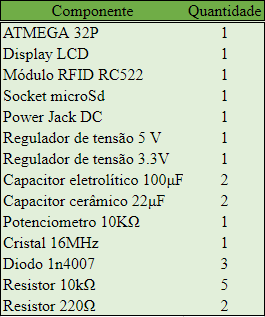
\includegraphics[scale=.7]{imagens/tabela_final}
	\\ \vspace{0.2cm}
	\textbf{Fonte:} Produzida pelos autores
	\label{tab:final}
\end{table}
\FloatBarrier


